
\section{Acquisition}

\begin{lstlisting}
Acquisition results for PRN ID 5
 Status:True Doppler:3500 Delay/Code-Delay:300/30.0
Acquisition results for PRN ID 7
 Status:True Doppler:2500 Delay/Code-Delay:587/58.7
Acquisition results for PRN ID 3
 Status:True Doppler:1500 Delay/Code-Delay:426/42.6
Acquisition results for PRN ID 1
 Status:True Doppler:2500 Delay/Code-Delay:313/31.3
\end{lstlisting}
\newpage
\section{Tracking and Decoding}
\textbf{Result}
\begin{lstlisting}
Tracking and decoding output for PRN ID:5
Transmitted Bits:
 [0. 1. 0. 1. 0. 0. 0. 1. 0. 1. 1. 0. 0. 0. 1. 1. 1. 0. 0. 1. 1. 1. 1. 0.1. 0. 1. 1. 0. 1. 0. 0. 1. 0. 0. 0. 1. 0. 1. 1. 1. 0. 1. 1. 0. 0. 1. 0. 0. 0.]
Received bits:
 [1. 1. 0. 1. 0. 1. 1. 1. 0. 1. 0. 0. 1. 1. 1. 0. 0. 0. 1. 1. 0. 0. 0. 0.1. 0. 1. 0. 0. 1. 0. 1. 1. 0. 1. 1. 1. 0. 1. 0. 0. 0. 1. 0. 0. 1. 1. 0.1. 1.]
Received bits inverted:
 [0. 0. 1. 0. 1. 0. 0. 0. 1. 0. 1. 1. 0. 0. 0. 1. 1. 1. 0. 0. 1. 1. 1. 1.0. 1. 0. 1. 1. 0. 1. 0. 0. 1. 0. 0. 0. 1. 0. 1. 1. 1. 0. 1. 1. 0. 0. 1. 0. 0.]
\end{lstlisting}
\begin{normalsize}
\begin{figure}[ht]
\centering
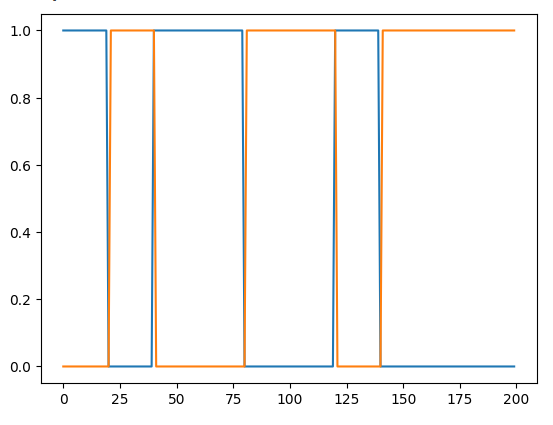
\includegraphics[width=1\columnwidth]{figs/tracking_plot.png}
\centering
\captionsetup{justification=centering}
\caption{Tracking result plot}
\label{fig:tracking_plot}
\end{figure}
\end{normalsize}






